\begin{examplebox}
\textbf{例1（轴上外点：直接化成二次式）。}

已知椭圆 $\dfrac{x^2}{9}+\dfrac{y^2}{4}=1$，
外点 $M(4,0)$，求 $M$ 到椭圆上点的距离极值。

\textbf{解：}设 $P=(3\cos\theta,2\sin\theta)$，
令 $u=\cos\theta$，则 $-1\le u\le1$。
\[
\begin{aligned}
MP^2&=(3\cos\theta-4)^2+4\sin^2\theta\\
    &=5u^2-24u+20.
\end{aligned}
\]
在 $[-1,1]$ 上，$10u-24<0$，故该式单调递减。
于是 $u=1$ 时 $MP_{\min}=1$，
$u=-1$ 时 $MP_{\max}=7$。
\[
\boxed{d_{\min}=1,\qquad d_{\max}=7.}
\]

\medskip
\textbf{例2（一般外点：万能代换）。}

仍取椭圆 $\dfrac{x^2}{9}+\dfrac{y^2}{4}=1$，
现取外点 $M(4,6)$，求距离极值。

由 $P=(3\cos\theta,2\sin\theta)$，
\[
MP^2=(3\cos\theta-4)^2+(2\sin\theta-6)^2.
\]
求导，极值条件为
\[
5\sin\theta\cos\theta
-12\sin\theta+12\cos\theta=0.
\]
令 $t=\tan\frac{\theta}{2}$，化为
\[
6t^4+17t^3+7t-6=0.
\]
因式分解：
\[
(2t-1)(t+3)(3t^2+t+2)=0.
\]
第三个因式判别式为 $-23<0$，
故实根为 $t=\frac12$ 或 $t=-3$。

对应候选点和距离：
\[
\begin{array}{c|c|c}
t & P & MP\\ \hline
\frac12 & (\frac95,\frac85) & \frac{11\sqrt5}{5}\\[3pt]
-3 & (-\frac{12}{5},-\frac65) & \frac{4\sqrt{145}}5
\end{array}
\]
另检查 $\theta=\pi$，即 $P=(-3,0)$：
$MP=\sqrt{85}$。
比较得
\[
\boxed{d_{\min}=\frac{11\sqrt5}{5},\qquad
       d_{\max}=\frac{4\sqrt{145}}5.}
\]

\medskip\textbf{例3（同例2，用法向量直接求最近点）。}
取 $a^2=9,b^2=4,M=(4,6)$，外点条件 $16/9+36/4>1$。
由法向量条件得
\[
4-x=\lambda x/9,\quad 6-y=\lambda y/4,
\]
所以 $x=36/(9+\lambda),\ y=24/(4+\lambda)$。
代入椭圆方程得
\[
\frac{144}{(9+\lambda)^2}+\frac{144}{(4+\lambda)^2}=1.
\]
观察 $\lambda=11$ 时，左边为 $144/400+144/225=9/25+16/25=1$。由正根唯一性，最近点为 $P_1=(9/5,8/5)$。
\[
MP_1^2=(4-9/5)^2+(6-8/5)^2=121/5,
\quad d_{\min}=11\sqrt5/5.
\]
若同时求最远点，观察 $\lambda=-24$ 也满足方程，且 $-24<-9$，由差值恒负的判定得 $P_2=(-12/5,-6/5)$ 为唯一最远点。
\[
MP_2^2=(32/5)^2+(36/5)^2=2320/25,
\quad d_{\max}=4\sqrt{145}/5.
\]
一般题目未必有容易观察出的根，可利用单调性夹逼最近点参数；本例的整数根只是便于演示。
% C083: extracted shared teaching figure.
\begin{center}
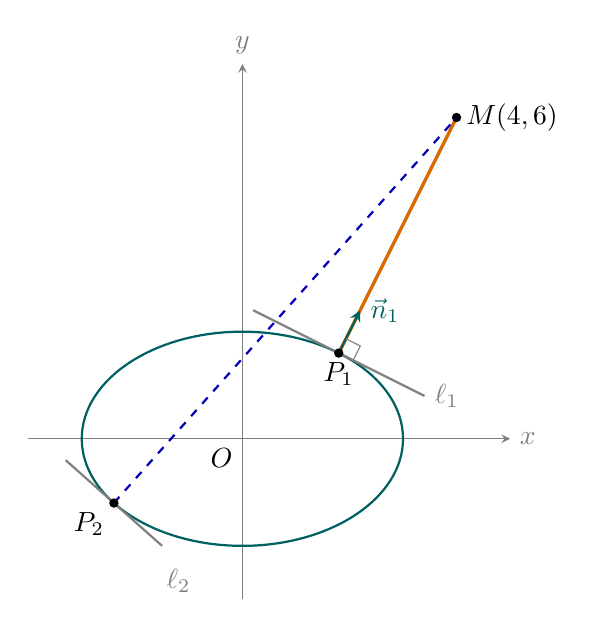
\begin{tikzpicture}[scale=.68,>=stealth]
\draw[->,gray] (-4,0)--(5,0) node[right]{$x$};
\draw[->,gray] (0,-3)--(0,7) node[above]{$y$};
\draw[teal!75!black,thick] (0,0) ellipse (3 and 2);
\coordinate (M) at (4,6); \coordinate (P) at (1.8,1.6);
\draw[orange!85!black,very thick] (P)--(M);
\draw[gray,thick] (.2,2.4)--(3.4,.8) node[right]{$\ell_1$};
\draw[->,teal!75!black,thick] (P)--(2.2,2.4) node[right]{$\vec n_1$};
\draw[gray] (2.068,1.466)--(2.202,1.734)--(1.934,1.868);
\fill (M) circle (2.5pt) node[right]{$M(4,6)$};
\fill (P) circle (2.5pt) node[below]{$P_1$};
\coordinate (R) at (-2.4,-1.2);
\draw[blue!70!black,dashed,thick] (R)--(M);
\draw[gray,thick] (-3.3,-.4)--(-1.5,-2.0);
\node[gray,anchor=north west] at (-1.6,-2.25) {$\ell_2$};
\fill (R) circle (2.5pt) node[below left]{$P_2$};
\node[below left] at (0,0) {$O$};
\end{tikzpicture}
\end{center}


\end{examplebox}
